% begin module arctan-def
\begin{frame}
\begin{columns}[c]
\column{.5\textwidth}
\ \only<handout:0| -1>{%
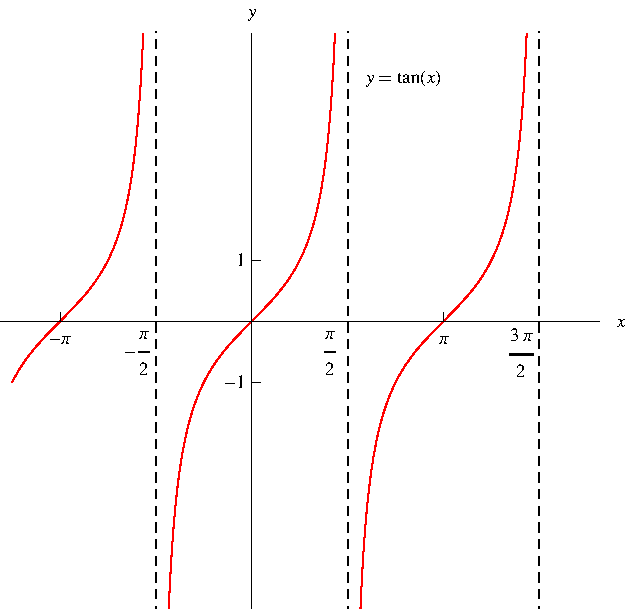
\includegraphics[width=5cm]{inverse-trig/pictures/07-06-arctana.pdf}%
}%
\only<handout:1| 2>{%
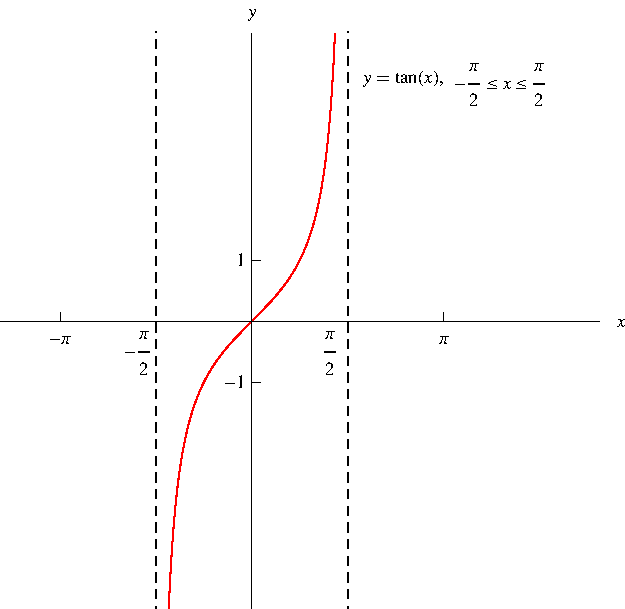
\includegraphics[width=5cm]{inverse-trig/pictures/07-06-arctanb.pdf}%
}%
\only<handout:2| 3->{%
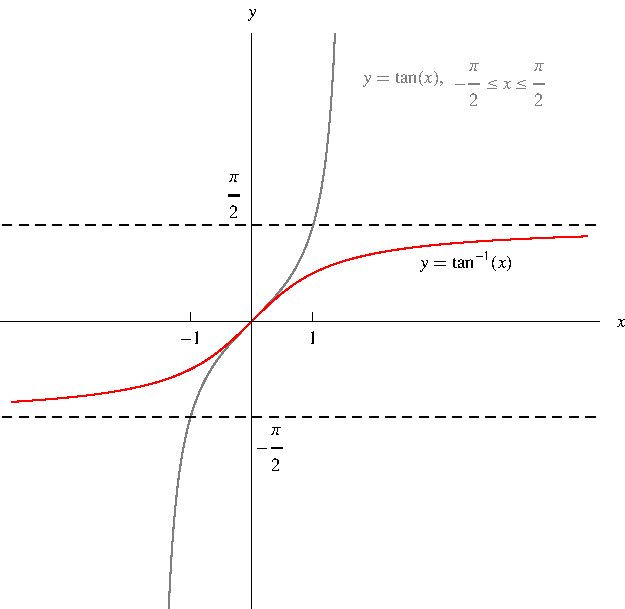
\includegraphics[width=5cm]{inverse-trig/pictures/07-06-arctanc.pdf}%
}%
\column{.5\textwidth}
\begin{itemize}
\item<1->  $\tan x$ isn't one-to-one.
\item<2->  Restrict the domain to $(-\pi /2, \pi /2)$.
\item<3->  The inverse is called $\arctan$ or $\tan^{-1}$.
\item<4->  $\arctan x = y \Leftrightarrow \tan y = x$ and $-\pi /2 < y < \pi /2$.
\item<5->  \alert<handout:0| 5-6>{Domain of $\arctan$: \uncover<6->{$(-\infty,\infty)$.}}
\item<5->  \alert<handout:0| 7-8>{Range of $\arctan$: \uncover<8->{$(-\pi / 2, \pi / 2)$.}}
\item<9->  \alert<handout:0| 9-10>{$\displaystyle \lim_{x\rightarrow \infty} \arctan x = \uncover<10->{\pi / 2.}$}
\item<9->  \alert<handout:0| 11-12>{$\displaystyle \lim_{x\rightarrow - \infty} \arctan x = \uncover<12->{- \pi / 2.}$}
\end{itemize}
\end{columns}
\end{frame}
% end module arctan-def
